\chapter{}
\label{lecture17}
Как мы уже говорили, для решения задачи о колебаниях мембраны методом Фурье надо найти собственные значения и собственные функции оператора Лапласа, что в явном возможно не при любой форме мембраны. Однако для прямоугольной и круглой мембраны это возможно. На прошлой лекции мы рассмотрели прямоугольную мембрану.
\section{Колебания круглой мембраны.}
\label{lecture17section1}
Пусть круглая мембрана радиуса $R$ расположена в плоскости $x,y$, её центр --- в точке $(0,0)$, края закреплены.
\begin{figure}[H]\centering
\tikzset{every picture/.style={line width=0.75pt}} %set default line width to 0.75pt        

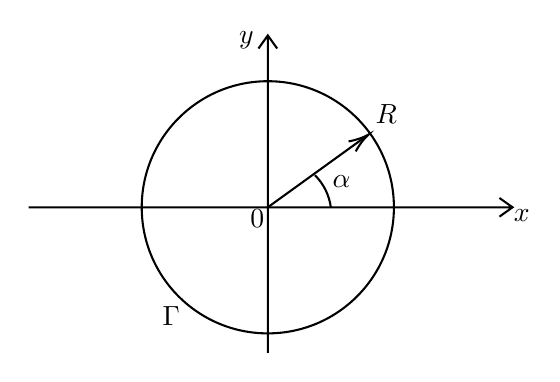
\begin{tikzpicture}[x=0.75pt,y=0.75pt,yscale=-0.9,xscale=0.9]
	%uncomment if require: \path (0,218); %set diagram left start at 0, and has height of 218
	
	%Shape: Axis 2D [id:dp2909137318191568] 
	\draw  (34,114) -- (293,114)(162,22) -- (162,192) (286,109) -- (293,114) -- (286,119) (157,29) -- (162,22) -- (167,29)  ;
	%Shape: Circle [id:dp6310794561218316] 
	\draw   (94.5,114) .. controls (94.5,76.72) and (124.72,46.5) .. (162,46.5) .. controls (199.28,46.5) and (229.5,76.72) .. (229.5,114) .. controls (229.5,151.28) and (199.28,181.5) .. (162,181.5) .. controls (124.72,181.5) and (94.5,151.28) .. (94.5,114) -- cycle ;
	%Straight Lines [id:da959835757179875] 
	\draw    (162,114) -- (214.38,76.17) ;
	\draw [shift={(216,75)}, rotate = 504.16] [color={rgb, 255:red, 0; green, 0; blue, 0 }  ][line width=0.75]    (10.93,-3.29) .. controls (6.95,-1.4) and (3.31,-0.3) .. (0,0) .. controls (3.31,0.3) and (6.95,1.4) .. (10.93,3.29)   ;
	%Shape: Arc [id:dp20537985491684618] 
	\draw  [draw opacity=0] (187.21,96.79) .. controls (191.82,101.39) and (194.93,107.48) .. (195.77,114.28) -- (166,118) -- cycle ; \draw   (187.21,96.79) .. controls (191.82,101.39) and (194.93,107.48) .. (195.77,114.28) ;
	
	% Text Node
	\draw (292,113.4) node [anchor=north west][inner sep=0.75pt]    {$x$};
	% Text Node
	\draw (145,18.4) node [anchor=north west][inner sep=0.75pt]    {$y$};
	% Text Node
	\draw (195,95.4) node [anchor=north west][inner sep=0.75pt]    {$\alpha $};
	% Text Node
	\draw (104,165.4) node [anchor=north west][inner sep=0.75pt]    {$\Gamma $};
	% Text Node
	\draw (218,57.4) node [anchor=north west][inner sep=0.75pt]    {$R$};
	% Text Node
	\draw (151,113.4) node [anchor=north west][inner sep=0.75pt]    {$0$};
	
	
\end{tikzpicture}
	\caption{~}
\label{l17:fig:1}
\end{figure}

\noindent Постановка задачи: найти функцию $u(x,y,t)$ являющуюся решением уравнения
\begin{equation}\label{l17:eq:1}
	 \pdder{u}{t}=a^2\cdot\Delta u
\end{equation}
с граничным условием
\begin{equation}\label{l17:eq:2}
	 u\Big|_{\Gamma}=0\qquad\left(\Gamma=\left\{x,y\middle|x^2+y^2=R^2\right\}\right)
\end{equation} 
и начальными условиями
\begin{equation}\label{l17:eq:3}
	u\Big|_{t=0}=\phi(x,y),\quad u_t\Big|_{t=0}=\psi(x,y).
\end{equation}
Отыскивая частное решение $u_{\text{ч}}=T(t)\cdot Z(x,y)$ задачи~\eqref{l17:eq:1},~\eqref{l17:eq:2} мы после разделения переменных приходим к уравнениям
\begin{equation}\label{l17:eq:4}
	 T''+a^2\cdot\lambda\cdot T=0,
\end{equation}
\begin{equation}\label{l17:eq:5}
	 -\Delta Z=\lambda\cdot Z.
\end{equation}
причём для функции $Z(x,y)$ должно выполняться в силу~\eqref{l17:eq:2} условия
\begin{equation}\label{l17:eq:6}
	 Z\Big|_{\Gamma}=0.
\end{equation}
Далее решаем задачу~\eqref{l17:eq:5},~\eqref{l17:eq:6}. Форма области позволяет сделать ещё одно разделение переменных, если ввести полярные координаты. Полагаем
\begin{equation}\label{l17:eq:7}
	 x=r\cdot\cos\alpha,\quad y=r\cdot\sin\alpha.
\end{equation} 
Отсюда 
\begin{equation}\label{l17:eq:8}
	 r=\sqrt{x^2+y^2},\quad\alpha=\arctg\frac{y}{x}.
\end{equation}
Пусть 
\begin{equation*}
	 v(r,\alpha)=Z(x,y)\quad\longleftrightarrow\quad\text{при условии~\eqref{l17:eq:7} (или~\eqref{l17:eq:8}).}
\end{equation*}
Подставим в $\Delta Z$ выражения производных от $Z$ через производные от $v(r,\alpha)$, которые, очевидно, выражаются следующим образом
\begin{multline*}
	\pder{Z}{x}=\pder{v}{r}\cdot\pder{r}{x}+\pder{v}{\alpha}\cdot\pder{\alpha}{x};\qquad\qquad\pdder{Z}{x}=\pder{r}{x}\cdot\left(\pdder{v}{r}\cdot\pder{r}{x}+\pder{^2v}{r\partial\alpha}\cdot\pder{\alpha}{x}\right)+\\
	+\pder{v}{r}\cdot\pdder{r}{x}+\pder{\alpha}{x}\cdot\left(\pder{^2v}{r\partial\alpha}\cdot\pder{r}{x}+\pdder{v}{\alpha}\cdot\pder{\alpha}{x}\right)+\pdder{\alpha}{x}\cdot\pder{v}{\alpha};
\end{multline*}
 $\displaystyle\pdder{Z}{y}$ записывается аналогично. Вычислив здесь $\displaystyle\pder{r}{x}$, $\displaystyle\pder{\alpha}{x}$, $\displaystyle\pdder{r}{x}$, $\displaystyle\pdder{\alpha}{x}$, $\displaystyle\pder{r}{y}$, $\displaystyle\pder{\alpha}{y}$, $\displaystyle\pdder{r}{y}$, $\displaystyle\pdder{\alpha}{y}$ увидим, что
\begin{equation*}
	-\Delta Z=-\frac{1}{r}\cdot\pder{}{r}\left(r\cdot\pder{v}{r}\right)-\frac{1}{r^2}\cdot\pdder{v}{\alpha}.
\end{equation*}
Подставляя это выражение в~\eqref{l17:eq:5}, получим 
\begin{equation}\label{l17:eq:9}
	-\frac{1}{r}\cdot\pder{}{r}\left(r\cdot v_r\right)-\frac{1}{r^2}\cdot\pdder{v}{\alpha}=\lambda\cdot v.
\end{equation}
Условие~\eqref{l17:eq:6} примет вид
\begin{equation}\label{l17:eq:10}
	 v\Big|_{r=R}=0.
\end{equation}

Будем искать функцию $v(r,\alpha)$ в виде произведения функций, одна из которых зависит только от $r$, а другая только от $\alpha$: $v(r,\alpha)=f(r)\cdot h(\alpha)$. Тогда~\eqref{l17:eq:9} запишется в виде
\begin{equation*}
	-\frac{1}{r}\cdot\pder{}{r}\left(r\cdot f'\right)\cdot h-\frac{f}{r^2}\cdot\pdder{h}{\alpha}=\lambda\cdot f\cdot h.
\end{equation*}
Поделив обе части этого уравнения на $f\cdot h$ и умножив на $r^2$, получим
\begin{equation}\label{l17:eq:11}
	-\frac{\displaystyle r\pder{}{r}(r\cdot f')}{f}-\frac{\displaystyle\pdder{h}{\alpha}}{h}=\lambda\cdot r^2.
\end{equation}
Так как при изменении $\alpha$ не меняется ни правая часть, ни первое отношение в~\eqref{l17:eq:11}, то отношение $h''/h$ не зависит от $\alpha$. Положим
\begin{equation}\label{l17:eq:12}
	-\frac{h''}{h}=\gamma,
\end{equation}
где $\gamma$ --- неизвестная константа. Из~\eqref{l17:eq:11} и~\eqref{l17:eq:12} следуют уравнения 
\begin{equation}\label{l17:eq:13}
	-r\cdot\pder{}{r}(r\cdot f')+\gamma\cdot f=\lambda\cdot r^2\cdot f
\end{equation}
и
\begin{equation}\label{l17:eq:14}
	-h''(\alpha)=\gamma\cdot h(\alpha).
\end{equation}
Из~\eqref{l17:eq:10} получим, что $h(\alpha)\cdot f(R)=0$, $\forall\alpha$ и, значит,
\begin{equation}\label{l17:eq:15}
	 f(R)=0.
\end{equation}
Для функции $h(\alpha)$ из естественных соображений должно выполняться условие периодичности 
\begin{equation}\label{l17:eq:16}
	 h(\alpha+2\cdot\pi)=h(\alpha).
\end{equation}
Найдём решения уравнения~\eqref{l17:eq:14} с условием~\eqref{l17:eq:16}, то есть периодические собственные функции и соответствующие собственные значения оператора $-\displaystyle\dder{}{\alpha}$. Умножая~\eqref{l17:eq:14} на $h(\alpha)$ скалярно в пространстве $\fL[{[0,2\cdot\pi]}]$, получим 
\begin{equation*}
	\int\limits_0^{2\cdot\pi}\!-\underbrace{\overline{h}(\alpha)}_{u}\cdot \underbrace{h''(\alpha)\,d\alpha}_{dv}=-h'(\alpha)\cdot\overline{h}(\alpha)\mathop{\Big|}\limits_{0}^{2\cdot\pi}+\int\limits_{0}^{2\cdot\pi}|h'(\alpha)|^2\,d\alpha=\gamma\cdot\int\limits_{0}^{2\cdot\pi}|h(\alpha)|^2\,d\alpha,
\end{equation*}
где $h'(2\cdot\pi)\cdot\overline{h}(2\cdot\pi)-h'(0)\cdot \overline{h}(0)=0$ в силу периодичности $h(\alpha)$. Следовательно, $\gamma\geqslant0$. Поэтому можно считать решения~\eqref{l17:eq:14} вещественными\footnote{Для комплексного $h(\alpha)=\widehat{h}(\alpha)+i\cdot\widetilde{h}(\alpha)$ вещественные функции $\widehat{h}(\alpha)$ и $\widetilde{h}(\alpha)$ были бы решениями~\eqref{l17:eq:14}.}. Далее, при $\gamma=0$ очевидное решение $h(\alpha)=C$. Считая далее $\gamma>0$, из~\eqref{l17:eq:14} получаем 
\begin{equation*}
	 h(\alpha)=c\cdot\cos\left(\sqrt{\gamma}\cdot\alpha\right)+d\cdot\sin\left(\sqrt{\gamma}\cdot\alpha\right).
\end{equation*} 
Запишем это решение в виде
\begin{equation*}
	 h(\alpha)=\sqrt{c^2+d^2}\cdot\sin\left(\sqrt{\gamma}\cdot\alpha+\delta\right),
\end{equation*}
где $\delta$ определяется из соотношений $\displaystyle \frac{c}{\sqrt{c^2+d^2}}=\sin\delta$, $\displaystyle \frac{d}{\sqrt{c^2+d^2}}=\cos\delta$. Из~\eqref{l17:eq:16} следует, что 
\begin{equation*}
	\sin\left(\sqrt{\gamma}\cdot\alpha+\sqrt{\gamma}\cdot2\cdot\pi+\delta\right)=\sin\left(\sqrt{\gamma}\cdot\alpha+\delta\right),
\end{equation*}
откуда
\begin{multline*}
	\sin\left(\sqrt{\gamma}\cdot\alpha+\sqrt{\gamma}\cdot 2\cdot\pi+\delta\right)-\sin\left(\sqrt{\gamma}\cdot\alpha+\delta\right)=\\=2\cdot\sin\left(\sqrt{\gamma}\cdot\pi\right)\cdot\cos\left(\sqrt{\gamma}\cdot\alpha+\delta+\sqrt{\gamma}\cdot\pi\right)=0
\end{multline*}
при $\forall\alpha$. Это возможно лишь при $\sqrt{\gamma}\cdot \pi=n\cdot \pi$, то есть при $\gamma=n^2$ и тогда 
\begin{equation*}
	 h(\alpha)=h_{n}(\alpha)=c_n\cdot\sin\left(n\cdot \alpha\right)+d_n\cdot\cos\left(n\cdot \alpha\right). 
\end{equation*} 
Таким образом собственному значению $\gamma=n^2$ оператора $\displaystyle-\dder{}{\alpha}$ при условии~\eqref{l17:eq:16} отвечают при $n>0$ две собственных функции, которые %после нормировки в $\displaystyle\fL[{[0,2\cdot\pi]}]$ 
мы обозначим 
\begin{equation*}
	 h_{n1}=\sin\left(n\cdot \alpha\right),\quad h_{n2}=\cos\left(n\cdot \alpha\right),
\end{equation*}
при $n=0$
\begin{equation*}
	 h_{01}=0,\quad h_{02}=1.
\end{equation*}
Подставим $\gamma=n^2$ в~\eqref{l17:eq:13} и перепишем~\eqref{l17:eq:13} в виде
\begin{equation}\label{l17:eq:17}
	-\der{}{r}\big(r\cdot f'\big)+\frac{n^2}{r}\cdot f=\lambda\cdot r\cdot f.
\end{equation}
Обозначим левую часть этого уравнения через $L(n)f$. Мы встречались с оператором $L(n)$ в~\cite{VI}, когда рассматривали задачу на минимум функционала специального вида 
\begin{equation*}
	\J[y]=\int\limits_{0}^{R}\left(x\cdot y'^2+\frac{\nu^2}{x}\cdot y^2\right)\,dx.\footnotemark{}
\end{equation*}\footnotetext{Сейчас $\nu^2=n^2$.}%
Мы выяснили, что~\eqref{l17:eq:17} --- это уравнение обобщённой задачи Штурма для оператора $L(n)$ в области $\mc{D}_{L}$ с условием~\eqref{l17:eq:15}. Обозначим через $\lambda_{nk}$ и $f_{nk}(r)$ --- соответственно собственные значения и собственные функции обобщённой задачи Штурма для оператора $L(n)$. Мы установили, что $\lambda_{nk}=\big(\mu_{nk}/R\big)^2$, где $\mu_{nk}$ --- это нули функции Бесселя первого рода $n$-ого порядка $J_n(\rho)$, а
\begin{equation*}
	 f_{nk}(r)=J_n\left(\frac{\mu_{nk}}{R}\cdot r\right),\quad k=1,2,\ldots
\end{equation*}  
Таким образом решение $v(r,\alpha)=f(r)\cdot h(\alpha)$ уравнения~\eqref{l17:eq:9} есть
\begin{equation}\label{l17:eq:18}
	 v_{nki}=f_{nk}\cdot h_{ni}=J_{n}\left(\frac{\mu_{nk}}{R}\cdot r\right)\cdot h_{ni}(\alpha).
\end{equation}
То есть собственные функции оператора $-\Delta$ в полярных координатах есть
\begin{equation*}
	 Z_{nki}(x,y)=v_{nki}(\rho,\alpha),
\end{equation*}
а соответствующие собственные значения $\displaystyle\lambda_{nk}=\left(\frac{\mu_{nk}}{R}\right)^2$. 

Подставим теперь $\lambda=\lambda_{nk}$ в уравнение~\eqref{l17:eq:4}, откуда, полагая $\omega_{nk}^2\?=a^2\cdot\lambda_{nk}$, получим
\begin{equation*}
	 T_{nk}(t)=A_{nk}\cdot\cos\left(\omega_{nk}\cdot t\right)+B_{nk}\cdot\sin\left(\omega_{nk}\cdot t\right).
\end{equation*}
Так как частное решение задачи есть произведение $T_{nk}(t)\cdot v_{nki}(r,\alpha)$, то неопределённые коэффициенты $A_{nk}$ и $B_{nk}$ в выражении $T_{nk}(t)$ могут зависеть от $i$ ($i=1,2$). Поэтому естественно положить 
\begin{equation*}
	 T_{nki}(t)=A_{nki}\cdot\cos\left(\omega_{nk}\cdot t\right)+B_{nki}\cdot\sin\left(\omega_{nk}\cdot t\right),
\end{equation*}
где $A_{nki}$ и $B_{nki}$ --- произвольные константы. 

 Таким образом, описываемое нами решение $u_{\text{ч}}=T_{nki}(t)\cdot v_{nki}(r,\alpha)$ (см.~\eqref{l17:eq:18}). Попробуем теперь найти решение~\eqref{l17:eq:1}--\eqref{l17:eq:3} в виде ряда 
\begin{equation}\label{l17:eq:19}
	 u=\sum\limits_{n=0}^{\infty}\sum\limits_{k=1}^{\infty}\sum\limits_{i=1}^{2}T_{nki}(t)\cdot v_{nki}(r,\alpha).
\end{equation}
Перейдём в начальных условиях к полярным координатам и пусть
\begin{equation*}
	\Phi(r,\alpha)=\phi(x,y),\quad F(r,\alpha)=\psi(x,y);
\end{equation*}
тогда условия~\eqref{l17:eq:3} запишутся в виде
\begin{equation*}
	 u(x,y,0)=\Phi(r,\alpha),\quad u_t(x,y,0)=F(r,\alpha)
\end{equation*}
и в силу~\eqref{l17:eq:19}
\begin{equation}\label{l17:eq:20}
	\sum\limits_{n=0}^{\infty}\sum\limits_{k=1}^{\infty}\sum\limits_{i=1}^{2}T_{nki}(0)\cdot v_{nki}(r,\alpha)=\Phi(r,\alpha),
\end{equation}
\begin{equation}\label{l17:eq:21}
	\sum\limits_{n=0}^{\infty}\sum\limits_{k=1}^{\infty}\sum\limits_{i=1}^{2}T'_{nki}(0)\cdot v_{nki}(r,\alpha)=F(r,\alpha).
\end{equation}
Перепишем эти соотношения,  подставляя в них   $T_{nki}(t)$ и $v_{nki}(r,\alpha)$:
\begin{multline}\label{l17:eq:22}
	\sum\limits_{n=0}^{\infty}\left\{\sum\limits_{k=1}^{\infty}\left[A_{nk1}\cdot J_n\left(\frac{\mu_{nk}}{R}\cdot r\right)\right]\cdot\sin\left(n\cdot\alpha\right)+\right.\\\left.\sum\limits_{k=1}^{\infty}\left[A_{nk2}\cdot J_n\left(\frac{\mu_{nk}}{R}\cdot r\right)\right]\cdot\cos\left(n\cdot\alpha\right) \right\}=\Phi(r,\alpha),
\end{multline}
\begin{multline}\label{l17:eq:23}
	\sum\limits_{n=0}^{\infty}\left\{\sum\limits_{k=1}^{\infty}\left[\omega_{nk}\cdot B_{nk1}\cdot J_n\left(\frac{\mu_{nk}}{R}\cdot r\right)\right]\cdot\sin\left(n\cdot\alpha\right)+\right.\\\left.+\sum\limits_{k=1}^{\infty}\left[\omega_{nk}\cdot B_{nk2}\cdot J_n\left(\frac{\mu_{nk}}{R}\cdot r\right)\right]\cdot\cos\left(n\cdot\alpha\right) \right\}=F(r,\alpha).
\end{multline}
Полагая 
\begin{equation}\label{l17:eq:24}
	\Phi_{ni}=\sum\limits_{k=1}^{\infty}A_{kni}\cdot J_{n}\left(\frac{\mu_{nk}}{R}\cdot r\right),\  F_{ni}=\sum\limits_{k=1}^{\infty}\omega_{nk}\cdot B_{nki}\cdot J_{n}\left(\frac{\mu_{nk}}{R}\cdot r\right),\quad i=1,2;
\end{equation}
видим, что разложение~\eqref{l17:eq:22} --- это разложение функции $\Phi(r,\alpha)$ при фиксированном $r$ в ряд Фурье
\begin{equation*}
	\sum\limits_{n=0}^{\infty}\Big(\Phi_{n1}(r)\cdot\sin\left(n\cdot\alpha\right)+\Phi_{n2}(r)\cdot\cos\left(n\cdot\alpha\right)\Big)=\Phi(r,\alpha),
\end{equation*}
а разложение~\eqref{l17:eq:23} --- аналогичное разложение для $F(r,\alpha)$:
\begin{equation*}
	\sum\limits_{n=0}^{\infty}\Big(F_{n1}(r)\cdot\sin\left(n\cdot\alpha\right)+F_{n2}(r)\cdot\cos\left(n\cdot\alpha\right)\Big)=F(r,\alpha),
\end{equation*}
где коэффициенты $\Phi_{ni}(r)$ и $F_{ni}(r)$ даются формулами
\begin{subequations}
	\label{l17:eq:25}
\begin{multline}\label{l17:eq:25a}
	\Phi_{n1}(r)=\frac{1}{\pi}\cdot\int\limits_{0}^{2\cdot\pi}\Phi(r,\alpha)\cdot\sin\left(n\cdot\alpha\right)\,d\alpha,\\
	\Phi_{n2}(r)=\frac{1}{\beta_n\cdot\pi}\cdot\int\limits_{0}^{2\cdot\pi}\Phi(r,\alpha)\cdot\cos\left(n\cdot\alpha\right)\,d\alpha,\quad n\geqslant0;
\end{multline}
\begin{multline}\label{l17:eq:25b}
	F_{n1}(r)=\frac{1}{\pi}\cdot\int\limits_{0}^{2\cdot\pi}F(r,\alpha)\cdot\sin\left(n\cdot\alpha\right)\,d\alpha,\\ F_{n2}(r)=\frac{1}{\beta_n\cdot\pi}\cdot\int\limits_{0}^{2\cdot\pi}F(r,\alpha)\cdot\cos\left(n\cdot\alpha\right)\,d\alpha,\quad n\geqslant0;
\end{multline}
\end{subequations}
где $\beta_n=1$ при $n\geqslant1$, $\beta_0=2$, то есть $\Phi_{01}(r)=F_{01}(r)=0$, а в $\Phi_{02}(r)$ и $F_{02}(r)$ в знаменателе $2\cdot\pi$ вместо $\pi$\footnote{$\pi$ и $2\cdot\pi$ --- это соответственно квадраты норм $\sin(n\cdot\alpha),\ \cos(n\cdot\alpha)$ при $n>0$ и $\cos(n\cdot\alpha)$ при $n=0$}.

Зная функции $\Phi_{ni}(r)$ и $F_{ni}(r)$ мы можем из~\eqref{l17:eq:24} найти неизвестные коэффициенты $A_{nki}$ и $B_{nki}$ на основании теоремы Стеклова. Как мы знаем из рассмотрения квадратичного функционала специального вида, функции $J_n\left(\dfrac{\mu_{nk}}{R}\cdot r\right)$ --- это собственные функции $y_{nk}(r)$ обобщённой задачи Штурма для оператора $L(n)$ из~\eqref{l17:eq:17} и по ним можно раскладывать функции из $\fLr[r;{[0,R]}]$; известно также, что они при разных $k$ ортогональны с весом $r$. Поэтому умножив равенства~\eqref{l17:eq:24} на $J_n\left(\dfrac{\mu_{nm}}{R}\cdot r\right)\cdot r$ и проинтегрировав по $r$ от $0$ до $R$, получим:
\begin{equation*}
	\begin{array}{rcl}
		\displaystyle\int\limits_{0}^{R}\Phi_{ni}(r)\cdot J_{n}\left(\frac{\mu_{nm}}{R}\cdot r\right)\cdot r\,dr&=&\displaystyle A_{nmi}\cdot\int\limits_{0}^{R}J_{n}^2\left(\frac{\mu_{nm}}{R}\cdot r\right)\cdot r\,dr,\\[18pt]
		\displaystyle \int\limits_{0}^{R}F_{ni}(r)\cdot J_{n}\left(\frac{\mu_{nm}}{R}\cdot r\right)\cdot r\,dr&=&\displaystyle\omega_{nm}\cdot B_{nmi}\cdot\int\limits_{0}^{R}J_{n}^2\left(\frac{\mu_{nm}}{R}\cdot r\right)\cdot r\,dr.
	\end{array}
\end{equation*} 
Из этих формул легко находятся константы $A_{nmi}$ и $B_{nmi}$\footnote{Напоминаю, что здесь $\Phi_{ni}(r)$ и $F_{ni}(r)$ даются равенствами~\eqref{l17:eq:25}.}. Таким образом задача о свободных колебаниях однородной круглой мембраны, закреплённой на границе, решена полностью.

Задача о вынужденных колебаниях под действием распределённой силы может быть решена по рецепту \hyperref[lecture15]{лекции~\ref{lecture15}} поскольку собственные функции $v_{nki}(r,\alpha)$ оператора Лапласа с нулевыми граничными условиями известны.

Рассмотрим вкратце задачу о \emph{колебаниях мембраны со свободной границей}. Вместо условия~\eqref{l17:eq:2} должно выполняться условие\setcounter{equation}{2}
\begin{equation}\label{l17:eq:2A}
	\left.\pder{u}{n}\right|_{\Gamma}=0.\tag{\theequation A}
\end{equation} 
Оно приводит к условиям~\eqref{l17:eq:6A}, \eqref{l17:eq:10A}, \eqref{l17:eq:15A}:\setcounter{equation}{6}%
\begin{equation}\label{l17:eq:6A}
	\left.\pder{z}{n}\right|_{\Gamma}=0,\tag{\theequation A}
\end{equation}\setcounter{equation}{10}%
\begin{equation}\label{l17:eq:10A}
	\left.\pder{v}{n}\right|_{\Gamma}=0,\tag{\theequation A}
\end{equation} \setcounter{equation}{15}%
\begin{equation}\label{l17:eq:15A}
	\left.\pder{f}{r}\right|_{z=R}=0.\tag{\theequation A}
\end{equation} \setcounter{equation}{25}%
Чтобы не вводить новых обозначений пусть по-прежнему $\lambda_{nk}$ и $f_{nk}(r)$~--- собственные значения и собственные функции обобщённой задачи Штурма для оператора $L(n)$, то есть для уравнения~\eqref{l17:eq:17}, но не с условием~\eqref{l17:eq:15}, а с условием~\eqref{l17:eq:15A}. Мы показывали в <<Лекциях по вариационному исчислению>>~\cite{VI}, что 
\begin{equation*}
	\lambda_{nk}=\left(\frac{\mu_{nk}'}{R}\right)^2,\quad f_{nk}(r)=J_n\left(\frac{\mu_{nk}'}{R}\cdot r\right),\quad k=1,2,\ldots,
\end{equation*}
где $\mu_{nk}'$ --- нули функции $\displaystyle J_n'(\rho)\eqdef\der{}{\rho}J_n(\rho)$. С учётом этого весь остальной ход решения сохраняется.
\begin{_rem}
	\hyperref[lecture18]{В следующей лекции}, где мы будем подробно изучать функции Бесселя и их свойства, будет повторён вывод формул для собственных значений и собственных функций задач~\eqref{l17:eq:17}, \eqref{l17:eq:15} и~\eqref{l17:eq:17},~\eqref{l17:eq:15A}.
\end{_rem}